%% \typeout{IJCAI--22 Instructions for Authors}

% These are the instructions for authors for IJCAI-22.

\documentclass{article}
\pdfpagewidth=8.5in
\pdfpageheight=11in
% The file ijcai22.sty is NOT the same as previous years'
\usepackage{ijcai23}

% Use the postscript times font!
\usepackage{times}
\usepackage{soul}
\usepackage{url}
\usepackage[hidelinks]{hyperref}
\usepackage[utf8]{inputenc}
\usepackage[small]{caption}
\usepackage{graphicx}
\usepackage{amsmath}
\usepackage{amsthm}
\usepackage{booktabs}
\usepackage{algorithm}
\usepackage{algorithmic}
\usepackage[switch]{lineno}
\linenumbers                    % comment this out for camera-ready
\urlstyle{same}
\usepackage{framed}
\newcommand{\highlight}[1]{\begin{framed}%
  \noindent\emph{#1}
\end{framed}}
%Custom in-text citation
\newcommand{\citet}[1]{\citeauthor{#1}~(\citeyear{#1})}

% the following package is optional:
%\usepackage{latexsym}

% See https://www.overleaf.com/learn/latex/theorems_and_proofs
% for a nice explanation of how to define new theorems, but keep
% in mind that the amsthm package is already included in this
% template and that you must *not* alter the styling.
\newtheorem{example}{Example}
\newtheorem{theorem}{Theorem}

% Following comment is from ijcai97-submit.tex:
% The preparation of these files was supported by Schlumberger Palo Alto
% Research, AT\&T Bell Laboratories, and Morgan Kaufmann Publishers.
% Shirley Jowell, of Morgan Kaufmann Publishers, and Peter F.
% Patel-Schneider, of AT\&T Bell Laboratories collaborated on their
% preparation.

% These instructions can be modified and used in other conferences as long
% as credit to the authors and supporting agencies is retained, this notice
% is not changed, and further modification or reuse is not restricted.
% Neither Shirley Jowell nor Peter F. Patel-Schneider can be listed as
% contacts for providing assistance without their prior permission.

% To use for other conferences, change references to files and the
% conference appropriate and use other authors, contacts, publishers, and
% organizations.
% Also change the deadline and address for returning papers and the length and
% page charge instructions.
% Put where the files are available in the appropriate places.

% PDF Info Is REQUIRED.
% Please **do not** include Title and Author information
\pdfinfo{
  /TemplateVersion (IJCAI.2023.0)
}

\title{Data vs. Model Machine Learning Fairness Testing: An Empirical Study}

% Single author syntax
%% \author{
%%     Author Name
%%     \affiliations
%%     Affiliation
%%     \emails
%%     pcchair@ijcai-22.org
%% }

% Multiple author syntax (remove the single-author syntax above and the \iffalse ... \fi here)

% \author{
%   Arumoy Shome$^1$
%   \and
%   Lu{\'\i}s Cruz$^1$\and
%   Arie van Deursen$^{1}$
%   \affiliations
%   $^1$Delft University of Technology\\
%   \emails
%   \{a.shome, l.cruz, arie.vandeursen\}@tudelft.nl
% }

\author{
Author(s)
\affiliations
Affiliation(s)
\emails
author(s)@example.org
}

\begin{document}

\maketitle

\begin{abstract}

  Preference has primarily been given to testing for robustness and
  correctness of ML systems while other non-functional properties such
  as fairness have been ignored. Although several fairness definitions
  and bias mitigation techniques exist in the literature, all existing
  solutions evaluate fairness after the training stage. This paper
  presents an empirical analysis of the relationship between model
  dependent and independent fairness metrics using $2$ fairness
  metrics, $4$ ML algorithms, $5$ real-world datasets and $1600$
  training and fairness evaluation cycles. We find a linear
  relationship between data and model fairness metrics when the
  distribution and the size of the training data changes. Our results
  indicate that testing for fairness prior to training can be a
  ``cheap'' and effective means of catching a biased data collection
  process early; detecting data drifts in production systems and
  minimising execution of full training cycles thus reducing
  development time and costs.

\end{abstract}

\section{Introduction}\label{sec:intro}

% Testing non-deterministic Machine Learning (ML) systems is
% challenging. 

% With ML being adopted in high-risk domains that have the
% ability to impact human lives, concerns are being raised toward trust,
% robustness, privacy, security and fairness of such systems. 

% The wide adoption of ML systems and its effect on human lives has
% prompted policy and law makers to include accountability and fairness
% in legislations for Artificial Intelligence (AI) systems through
% policies such as the \emph{General Data Protection Regulation (2018)}
% and more recently \emph{The Artificial Intelligence Act
% (2021)}. 

While several contributions toward testing ML systems have been made
in recent years, preference has primarily been given to robustness and
correctness while other non-functional properties such as security,
privacy, efficiency, interpretability and fairness have been
ignored \cite{zhang2020machine,zhang2021ignorance,mehrabi2021survey,wan2021modeling}. Testing
for fairness in ML systems however, is a multi-faceted problem and
involves both technological and social factors. Although an abundance
of definitions for fairness and consequently techniques to mitigate
said bias exists in the scientific literature, all existing solutions
evaluate fairness after the training stage, using the predictions of
the ML model.

In addition to the underlying codebase of ML software systems, both
the training data and the ML algorithms constantly evolve and change
throughout the ML development
lifecycle \cite{sculley2015hidden,bosch2021engineering,hutchinson2021towards}. In
contrast to prior work, we take a more holistic approach by testing
for fairness at two distinct locations of the ML development
lifecycle. First, prior to model training using fairness metrics that
can quantify the bias in the training data (henceforth Data Fairness
Metric or DFM). And second, after model training using fairness
metrics that quantify the bias in the predictions of the trained model
(henceforth Model Fairness Metric or MFM).

This paper presents an empirical study of the relationship between DFM
and MFM. The analysis is conducted using $2$ fairness metrics, $4$ ML
algorithms, $5$ real-world tabular datasets and $1600$ fairness
evaluation cycles. All source code and results of the study are
publicly accessible under the CC-BY 4.0
license\footnote{https://figshare.com/s/67206f7c219b12885a6f}. The
research questions along with the contributions of this paper are as
follows.

\begin{itemize}
  \item{\textbf{RQ1.}} What is the relationship between DFM and MFM as the
    fairness properties of the underlying training dataset changes?

    DFM and MFM convey the same information when the distribution of
    the underlying training dataset changes. This implies that DFM can
    be used as early warning systems to catch data drifts in
    production ML systems that may affect its fairness.

  \item{\textbf{RQ2.}} How does the training sample size affect the
    relationship between DFM and MFM?

    Our analysis of the training sample size and how it influences the
    relationship between DFM and MFM reveals the presence of
    a trade-off between fairness, efficiency and performance. In
    Section \ref{sec:discuss} we provide some practical guidelines on
    how to best navigate this trade-off.

  \item{\textbf{RQ3.}} What is the relationship between DFM and MFM across
    various training and feature sample sizes?

    DFM and MFM convey the same information when the training sample
    size changes. This implies that DFM can help practitioners catch
    fairness issues upstream and avoid execution costs of a full
    training cycle.
\end{itemize}

The remainder of the paper is structured as follows.
Section \ref{sec:related} summarises related concepts and prior work
done in the field of ML fairness testing. In Section \ref{sec:method},
the experimental design and fairness evaluation strategy is presented.
The results of this study are presented in Section \ref{sec:results}.
The implications of the results along with their threats to validity
are discussed in Section \ref{sec:implications}.

\section{Preliminaries}\label{sec:related}

This section provides a summary of the relevant concepts and prior
work done in ML fairness testing.

\subsection{Algorithmic Bias, Bias Mitigation and Group Fairness}\label{sec:bias-fairness}

% Determining what is fair is a difficult problem under any social,
% political or economical circumstance. Fairness in the context of ML is
% no different and currently an open challenge. 

Manually validating the fairness of the labels is often an expensive
and time consuming process which is still prone to cognitive and
social biases of the human auditors. Significant efforts have
therefore been made to quantify the bias present in a ML model using
fairness metrics. Existing fairness metrics are restricted to
supervised binary classification problems where one of the outcomes is
more favourable than the other and the dataset contains one or more
\emph{protected attributes} such as \emph{race, sex, age, colour,
religion or disability status}. An ML model is said to make unfair
decisions if it favours a certain group or individual pertaining to
one or more protected attributes in the dataset.

Fairness metrics can be broadly classified into two
categories---namely, \emph{group fairness} and \emph{individual
fairness}. Individual fairness dictates that the predictions of an ML
model should not differ for two individuals who only differ in the
value of the protected attribute. While group fairness dictates that
the predictions of an ML model should be similar for both privileged
and unprivileged groups present in the
dataset \cite{castelnovo2022clarification,hellman2020measuring,mitchell2021algorithmic,kusner2017counterfactual,grgic2016case,dwork2012fairness,barocas2019fairness,barocas2016big,hardt2016equality,binns2018fairness,verma2018fairness,saxena2019fairness}.

Once an appropriate definition of fairness is identified, the relevant
techniques to mitigate said bias must be found. Bias mitigation
techniques can be classified into three groups based on the location
where the mitigation technique is applied: \emph{pre-processing,
in-processing and post-processing}. Several in-processing techniques
or novel ML algorithms have been proposed that take fairness into
consideration while training from biased
data \cite{zhang2018mitigating,agarwal2018reductions,kearns2018preventing,kamishima2012fairness}. In
contrast to in-processing techniques which target the ML model,
pre-processing
 \cite{feldman2015certifying,zemel2013learning,calmon2017optimized,kamiran2012data}
and post-processing
 \cite{pleiss2017fairness,hardt2016equality,kamiran2012decision}
techniques are applied to the training data and the predictions of the
ML model respectively.

This study uses group fairness metrics due to their popularity in
existing empirical studies on ML fairness testing and ease of
understandability \cite{zhang2021ignorance,biswas2020machine,biswas2021fair,hort2021fairea,chakraborty2021bias}. Our
analysis of the relationship between the DFM and MFM (see
Section \ref{sec:discuss}) presents practical guidelines for
practitioners to pick the appropriate bias mitigation strategy based
on the particular fairness issue they are facing.

\subsection{Prior Work in ML Fairness Testing}\label{sec:prior-work}

There is a growing consensus amongst academics that not all fairness
metrics can be satisfied simultaneously. There is also a consensus
that fairness and performance of ML systems are orthogonal to one
another and involve a trade-off. In fact, identifying the correct
fairness metric is the primary challenge which typically depends on
the domain and problem at hand. It is therefore recommended to
consider fairness as early as the requirements engineering and
software design
phase \cite{zhang2020machine,chen2022fairness,mehrabi2021survey,zhang2021ignorance}.

Several literature surveys have been conducted to classify and
catalogue various ML fairness testing and bias mitigation techniques.
\citeauthor{wan2021modeling} conducted a large scale survey on
in-processing bias mitigation strategies and their effectiveness.
\citeauthor{chen2022fairness} and \citeauthor{mehrabi2021survey}
conducted a survey of existing literature on fairness testing in ML
systems. \citeauthor{mehrabi2021survey} present a comprehensive survey
on the state-of-the-art research on fairness in ML with an emphasise
on fairness issues arising from both the data and the model.
\citeauthor{chen2022fairness} survey 113 papers addressing fairness
testing and provide a formal definition of fairness bugs and fairness
testing in ML from a software engineering perspective. Authors also reflect on how
fairness testing differs from traditional software testing and provide
practical guidelines on how and where to test for fairness within the
entire Software Development
Lifecycle \cite{wan2021modeling,chen2022fairness,mehrabi2021survey}.

Prior work has also focused on conducting empirical analysis of bias
mitigation techniques. \citeauthor{biswas2021fair} take a holistic
view of the entire ML pipeline and analyse the effect of common data
pre-processing techniques such as standardisation, feature selection,
encoding and sampling on the fairness of ML models. The analysis is
conducted using 37 real-world ML pipelines from Kaggle notebooks which
operate on five datasets. Typically data for the unprivileged group
tends to be limited which make pre and post processing bias mitigation
techniques less effective. \citeauthor{feffer2022empirical} thus
conduct an empirical analysis of bias mitigation in combination with
popular ensemble techniques to understand the effectiveness of such
combinations. \citeauthor{zhang2021ignorance} studied the effect of
training sample and feature sample size on the fairness of ML
models. Authors observe that a large feature sample combined with
a small training set helps reduce
bias \cite{biswas2021fair,feffer2022empirical,zhang2021ignorance}.

Prior work discussed so far operate under the assumption that the
training data and learning algorithm are accessible to the ML
practitioner---often referred to as \emph{white-box testing}. In
contrast, \emph{black-box testing} makes no such assumptions and
treats the entire ML pipeline as a black-box where we can only control
the input to the system and see the corresponding output. For such
situations, several test input generation techniques have been
proposed. \citeauthor{galhotra2017fairness} proposed \emph{Themis},
a tool which automatically generates a testing suite to measure
discrimination in software using causal fairness
testing. \citeauthor{udeshi2018automated} propose \emph{Aequitas}, an
automated tool that accepts a model and the protected attributes as
input and explores the input space to detect specific examples that
may produce discriminatory behaviour in the
model. \citeauthor{aggarwal2019black} propose a new technique for
generating test input using symbolic execution which accounts for
correlation amongst the protected and unprotected
attributes \cite{aggarwal2019black,udeshi2018automated,galhotra2017fairness}.

% Removing protected attributes prior to training (often referred to as
% \emph{fairness through unawareness}) is a naive solution which does
% not work when the protected and unprotected attributes are correlated
% to one another. Themis and Aequitas generate random test suites to
% measure presence of individual bias in the model. However they do not
% consider the correlation between protected and unprotected attributes
% and thus often miss such cases. 

This study conducts an empirical analysis of the relationship between
DFM and MFM, and as such, operates under white-box testing
assumptions. The experimental design of this study is similar in
spirit to that proposed by \citet{zhang2021ignorance}. However our
objective, results and implications are entirely different. While
\citet{zhang2021ignorance} study the effect of training and feature
sample size on the fairness of the model, this study aims to
understand the relationship between DFM and MFM. We analyse how change
in the distribution, sample size and number of features in the
training set affects this relationship.

\section{Experimental Design}\label{sec:method}

This section presents the datasets, ML models and fairness metrics
used in this study followed by the methodology used to evaluate DFM
and MFM.

\subsection{Datasets, ML Models and Fairness Metrics}\label{sec:method-parameters}

\begin{table}
  \centering
  \begin{tabular}{l r}
    \toprule
    \textbf{\emph{DFM}}\\
    \midrule
    DI & \(\displaystyle \frac{P(Y=1|D=0)}{P(Y=1|D=1)}\)\\
    SPD & \(\displaystyle P(Y=1|D=0)-P(Y=1|D=1)\)\\
    \midrule
    \textbf{\emph{MFM}}\\
    \midrule
    DI & \(\displaystyle \frac{P(\hat{Y}=1|D=0)}{P(\hat{Y}=1|D=1)}\)\\
    SPD & \(\displaystyle P(\hat{Y}=1|D=0)-P(\hat{Y}=1|D=1)\)\\
    \bottomrule
  \end{tabular}
  \caption{Fairness metrics used in this study}
  \label{tab:fairness-metrics}
\end{table}

Table \ref{tab:fairness-metrics} shows the group fairness metrics
along with their mathematical formulas used in this study. We include
all group fairness metrics---namely \emph{Disparate Impact (DI)} and
\emph{Statistical Parity Difference (SPD)}---for which both model
dependent and independent variants are available. The DFM use the
labels of the data ($Y$) where as the MFM use the predictions of the
trained ML models ($\hat{Y}$). Favourable and unfavourable outcomes
are represented by $1$ and $0$ respectively. Similarly, privileged and
unprivileged groups of the protected attribute ($D$) are represented
by $1$ and $0$ respectively. All fairness metrics and datasets used in
this study are obtained from the \emph{AIF360} python
library \cite{bellamy2019ai}.

\begin{table}
  \centering
  \begin{tabular}{l l r}
    \toprule
    \textbf{Name} & \textbf{Prot.} & \textbf{\#Eg.}\\
    \midrule
    German \cite{hofmann1994german} & age, sex & 1000\\
    Compas\cite{angwin2016machine} & race, sex & 6167\\
    MEPS \cite{mepsdata} & race & 15675\\
    Bank\cite{moro2014data} & age & 30488\\
    Adult\cite{kohavi1996scaling} & race, sex & 45222\\
    \bottomrule
  \end{tabular}
  \caption{Datasets used in the study}
  \label{tab:datasets}
\end{table}

Table \ref{tab:datasets} presents the datasets used in this study. We
consider tabular datasets which have been extensively used in prior
scientific contributions on ML fairness
testing \cite{zhang2021ignorance,biswas2020machine,biswas2021fair,chen2022fairness}. Based
on prior work, we only consider one protected attribute at any given
time thus giving us eight independent datasets. We follow the default
pre-processing steps implemented in the AIF360 library---missing
values are dropped and categorical features are label encoded. Prior
to training, the features in the training and testing subsets are
standardised by removing the mean of the sample and scaling to unit
variance.

We use the scikit-learn \cite{pedregosa2011scikit} python library for
creating the train-test splits and training the ML models. We use four
ML models of varying complexity namely, \emph{Logistic Regression},
\emph{Decision Trees}, \emph{Random Forest} and \emph{Ada boost} based
on their popularity in practise and in prior scientific
publications \cite{zhang2021ignorance,biswas2021fair,biswas2020machine}.

\subsection{Fairness Evaluation}\label{sec:method-fair-eval}

Figure \ref{fig:method} presents the methodology used in this study
for evaluating the fairness of ML models and datasets. A 75--25 split
with shuffling is used to create the training and testing splits. DFMs
and MFMs are used to quantify the bias in the underlying distribution
of the training set and the predictions of the models respectively. We
adopted the transformation steps from prior work to scale all fairness
metric values between $0$ and $1$ such that higher values indicate
more bias \cite{zhang2021ignorance,hort2021fairea}.

\begin{figure*}
  \centering
  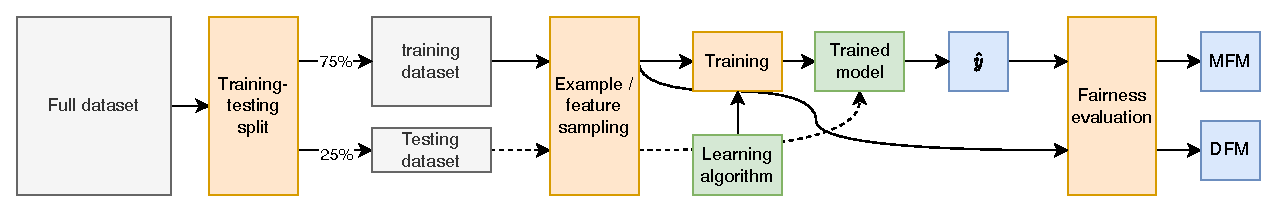
\includegraphics[width=\linewidth]{method.pdf}
  \caption{Methodology for evaluating fairness of datasets and ML
  models using DFM and MFM.}
  \label{fig:method}
\end{figure*}

We extend the above experiment further in two ways. First, we
experiment with different number of examples and second with different
number of features in the training set. For both experiments, we
shuffle the order of the examples in the training and testing
sets. Additionally, for the feature sample size experiment we shuffle
the order of the features.

For the training sample size experiment, we generate different
training samples of varying sizes starting from 10\% of the original
training data, and increase in steps of 10\% until the full quantity
is reached. For the feature sample size experiment, we start with
a minimum of three features (in addition to the protected attribute
and target) and introduce one new feature until all the features are
utilised. Both the training and testing sets undergo the same feature
sampling procedure in the feature sample size experiment. No such
sampling is done in the testing set for the training sample size
experiment.

\begin{table}
  \centering
  \begin{tabular}{l r}
    \toprule
    \textbf{Parameter} & \textbf{Count}\\
    \midrule
    Fairness metrics & $2$\\
    ML models & $4$\\
    Datasets & $8$\\
    Total cases & $8\times4=32$\\
    Iterations & $50$\\
    Total fairness evaluation cycles & $32\times50=1600$\\
    \bottomrule
  \end{tabular}
  \caption{Parameters of the study}
  \label{tab:parameters}
\end{table}

We use Spearman Rank Correlation to quantify the linear relationship
between the DFM and MFM. We repeat all experiments 50 times and report
the statistical significance of our results. We consider cases where
$pvalue\le0.05$ to be statistically significant in our
evaluation. Table \ref{tab:parameters} summarises the parameters of
the study. We train 4 ML models on 8 datasets producing 32 total
cases. The fairness for each case is evaluated 50 times using two
fairness metrics, thus producing a total of 1600 training and fairness
evaluation cycles.

\section{Results}\label{sec:results}

This section presents the analysis of the relationship between DFM and
MFM. The section is broken into two
subsections. Section \ref{sec:results-full} presents the relationship
between DFM and MFM as the distribution of the training data changes
while Section \ref{sec:results-training-feature-sets} presents their
relationship across varying training and feature sample sizes.

\subsection{Full Training Set Experiments}\label{sec:results-full}
\subsubsection{RQ1. What is the relationship between DFM and MFM as
the fairness properties of the underlying training dataset changes?}\label{sec:results-full-rel}

\begin{figure}
  \centering
  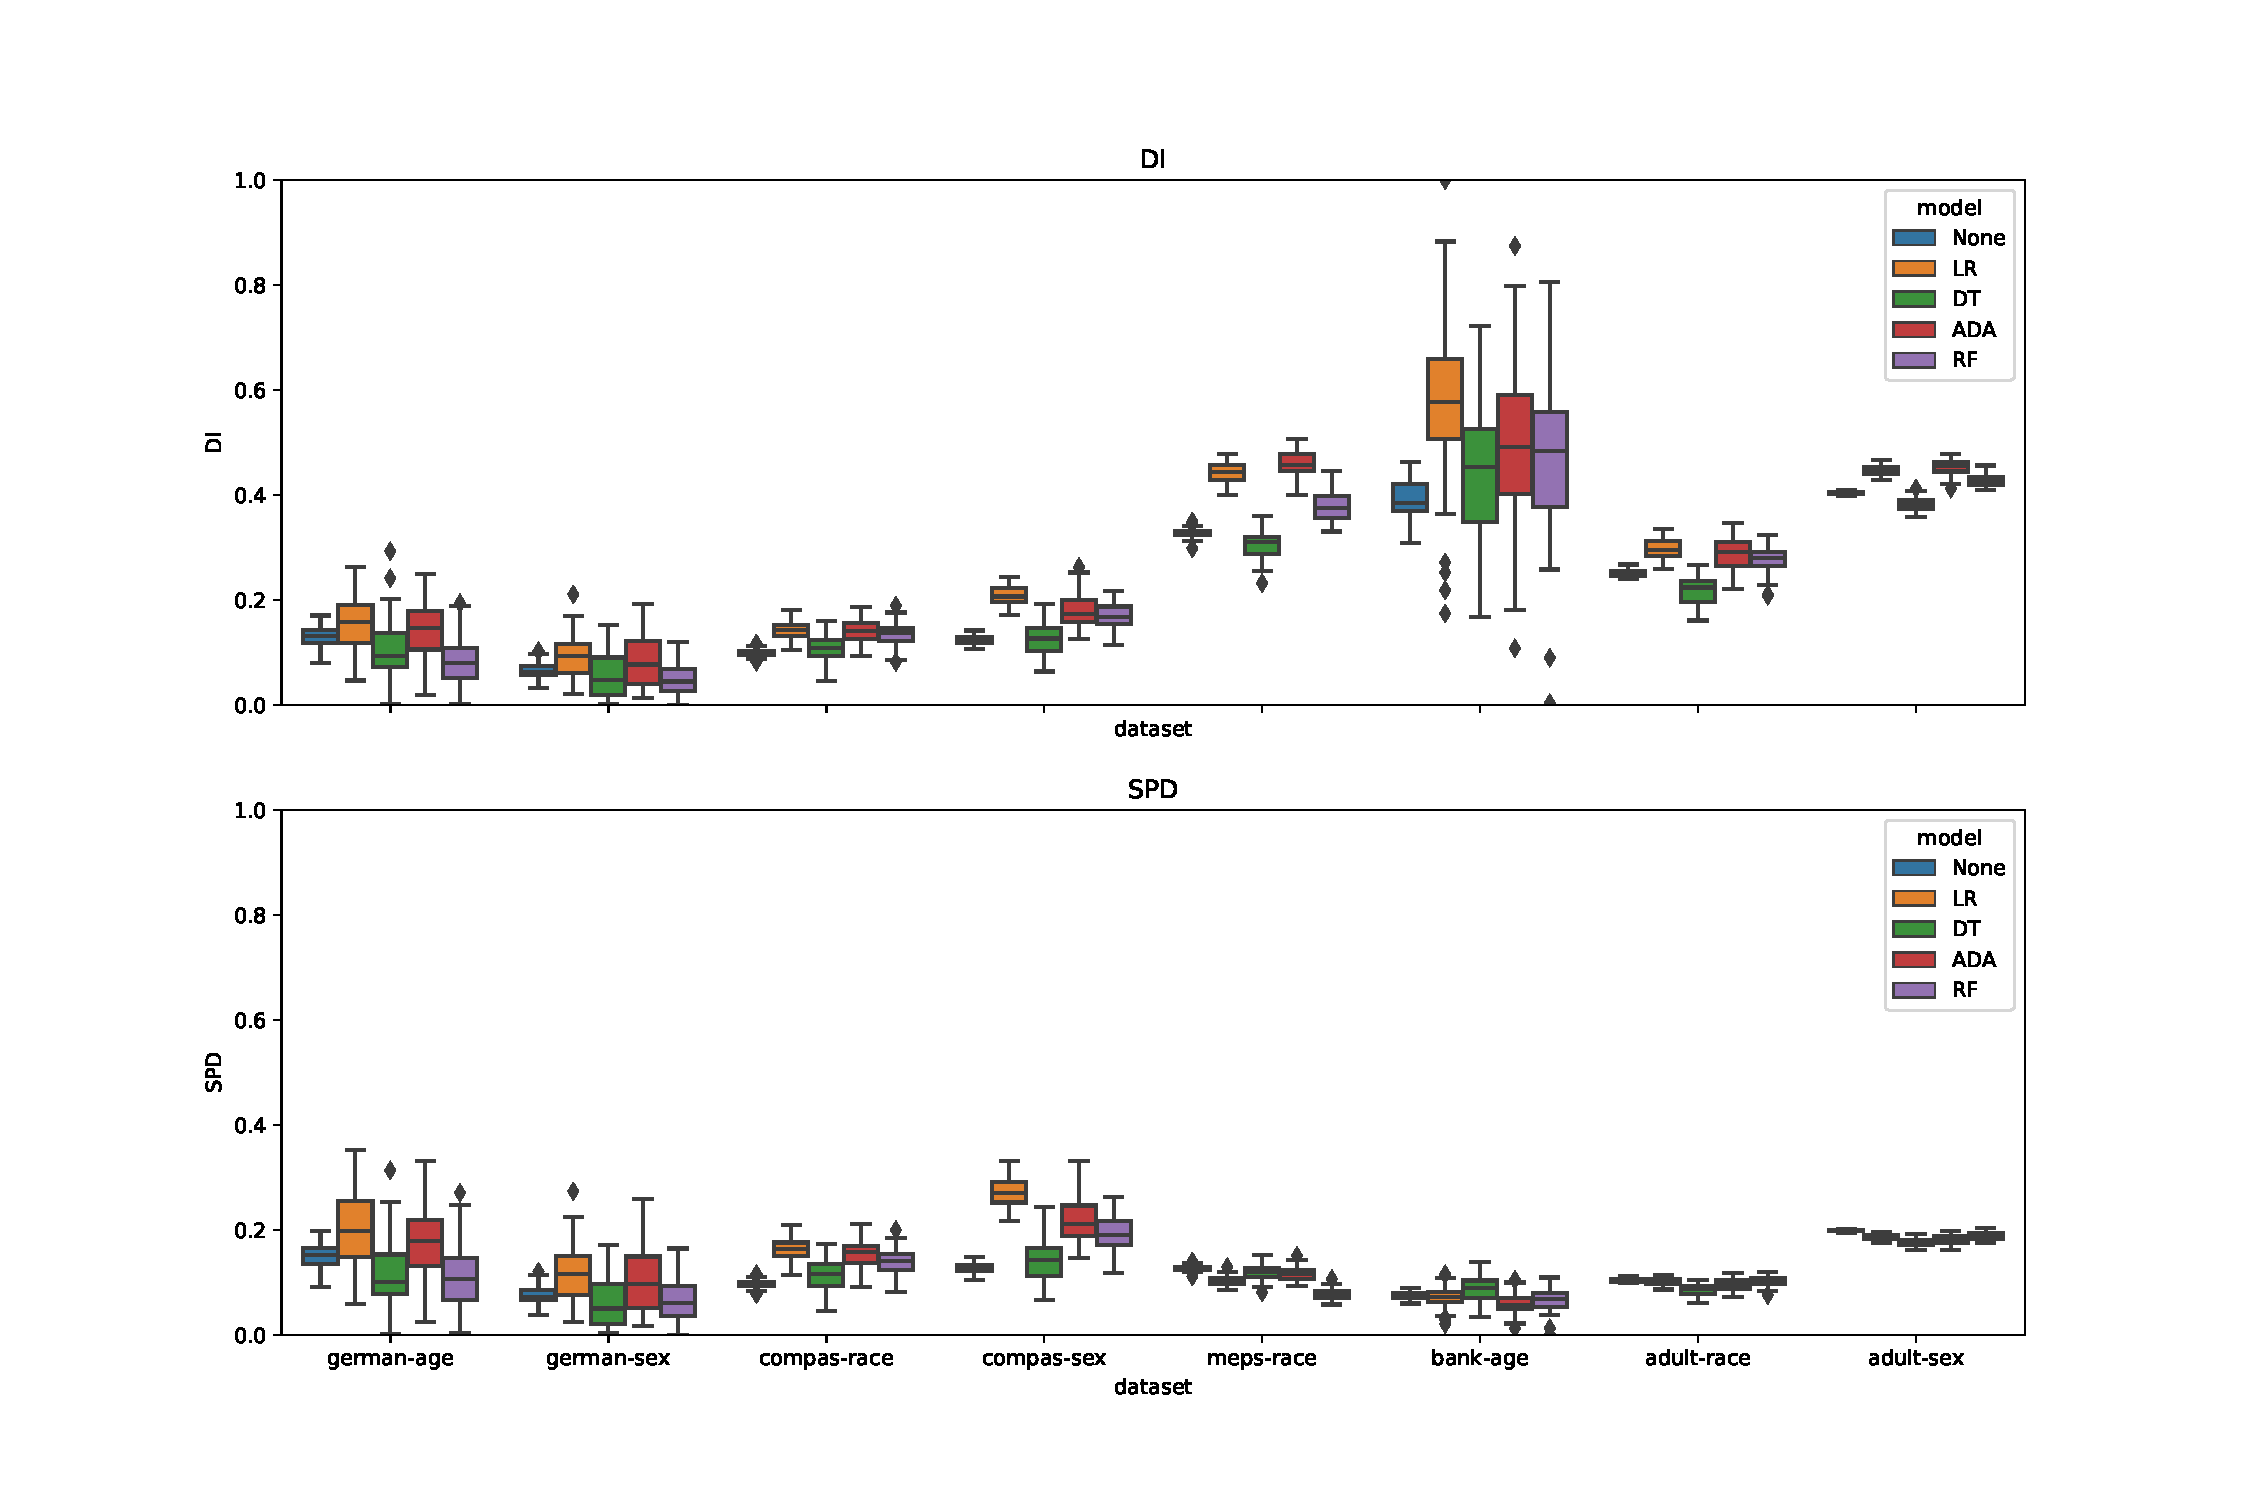
\includegraphics[width=\linewidth]{boxplot--dataset--di-spd--exp-full.pdf}
  \caption{Distribution of DFM and MFM across all datasets and models.}
  \label{fig:boxplot--dataset--di-spd--exp-full}
\end{figure}

Figure \ref{fig:boxplot--dataset--di-spd--exp-full} presents a boxplot
with the distribution of the fairness metrics across the datasets. The
x-axis represents the datasets used in this study while the y-axis
presents the value of the fairness metric. The models used in this
study are represented using different colors---note that the model
``None'' represented in blue refers to the DFM. Both the fairness
metrics DI (top) and SPD (bottom) are presented in separate plots. We
observe that distribution of the DFM and MFM are similar in all cases
indicating that they convey similar information. The variability of
the DFM is less than the MFM. This is because in addition to the
randomness from the data shuffling in the training set, the models are
assigned random initial states in every iteration. Finally in several
cases the tree-based classifiers (DT and RF) make fairer decisions
compared to the other classifiers, sometimes even better than the
baseline provided by the DFM.

\begin{figure}
  \centering
  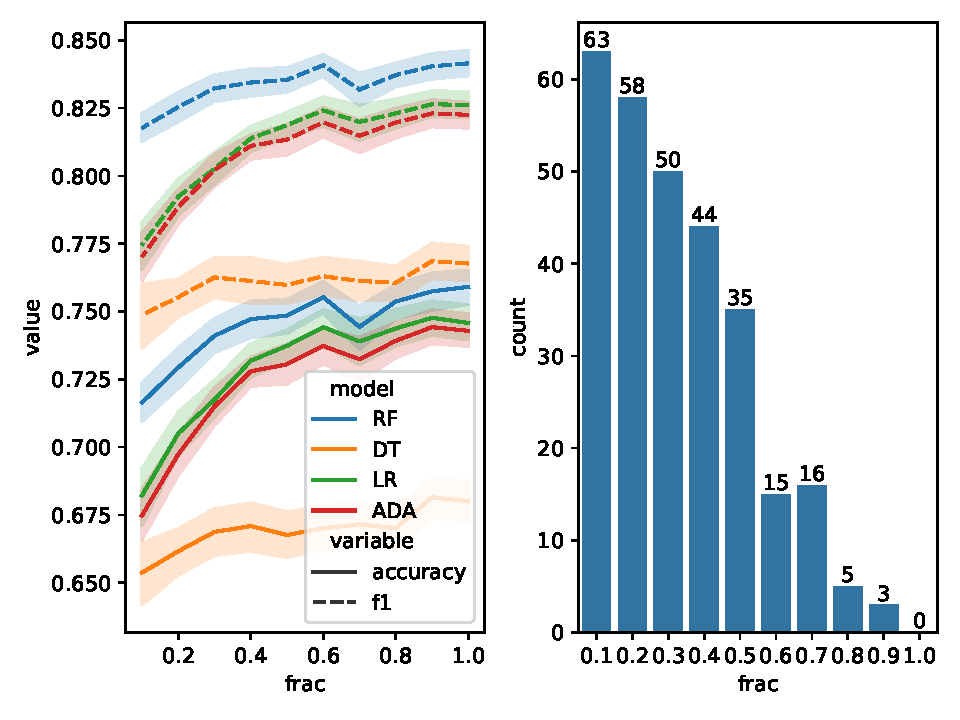
\includegraphics[width=0.95\linewidth]{training-set-frac-threshold.pdf}
  \caption{\emph{\textbf{(left)}} Accuracy and f1 across various
  training sample size in the german-age
  dataset. \emph{\textbf{(right)}} Count of cases with significant
  change in accuracy and f1.}
  \label{fig:training-set-frac-threshold}
\end{figure}

To analyse the relationship between the DFM and MFM across various
data distributions, we calculate the DFM and MFM across training
samples of varying size. The data distribution in smaller training
samples will change more frequently in the 50 iterations at the loss
of data quality. To identify a sample size that captures a variety of
data distribution changes while also being a realistic training
dataset, we analyse the \emph{accuracy} and \emph{f1 score} of the
models across the training sample sizes. Next, we conduct
\emph{student t-test} to identify the smallest sample size where the
performance of the models is similar to that obtained when trained
using the full training set.

Figure \ref{fig:training-set-frac-threshold} (right) presents
a histogram of the number of cases where there was a significant
difference between the two populations. We note that there is
a significant difference in the performance of the models in the
majority of the cases when the training size is reduced to 50\% while
it remains consistent when using a training size of 60\% or
higher. This is also corroborated by the lineplot in
Figure \ref{fig:training-set-frac-threshold} (left) which shows the
accuracy and f1 of all models across various training sample sizes in
the \emph{german-age} dataset. We observe that the performance
stabilises starting from 60\% training sample size. Thus for the
majority of the cases, a training sample of 60\% allows us to train
models with acceptable performance, while also capturing a wide
variety of fairness issues in the underlying training data within the
50 iterations.

\begin{figure}
  \centering
  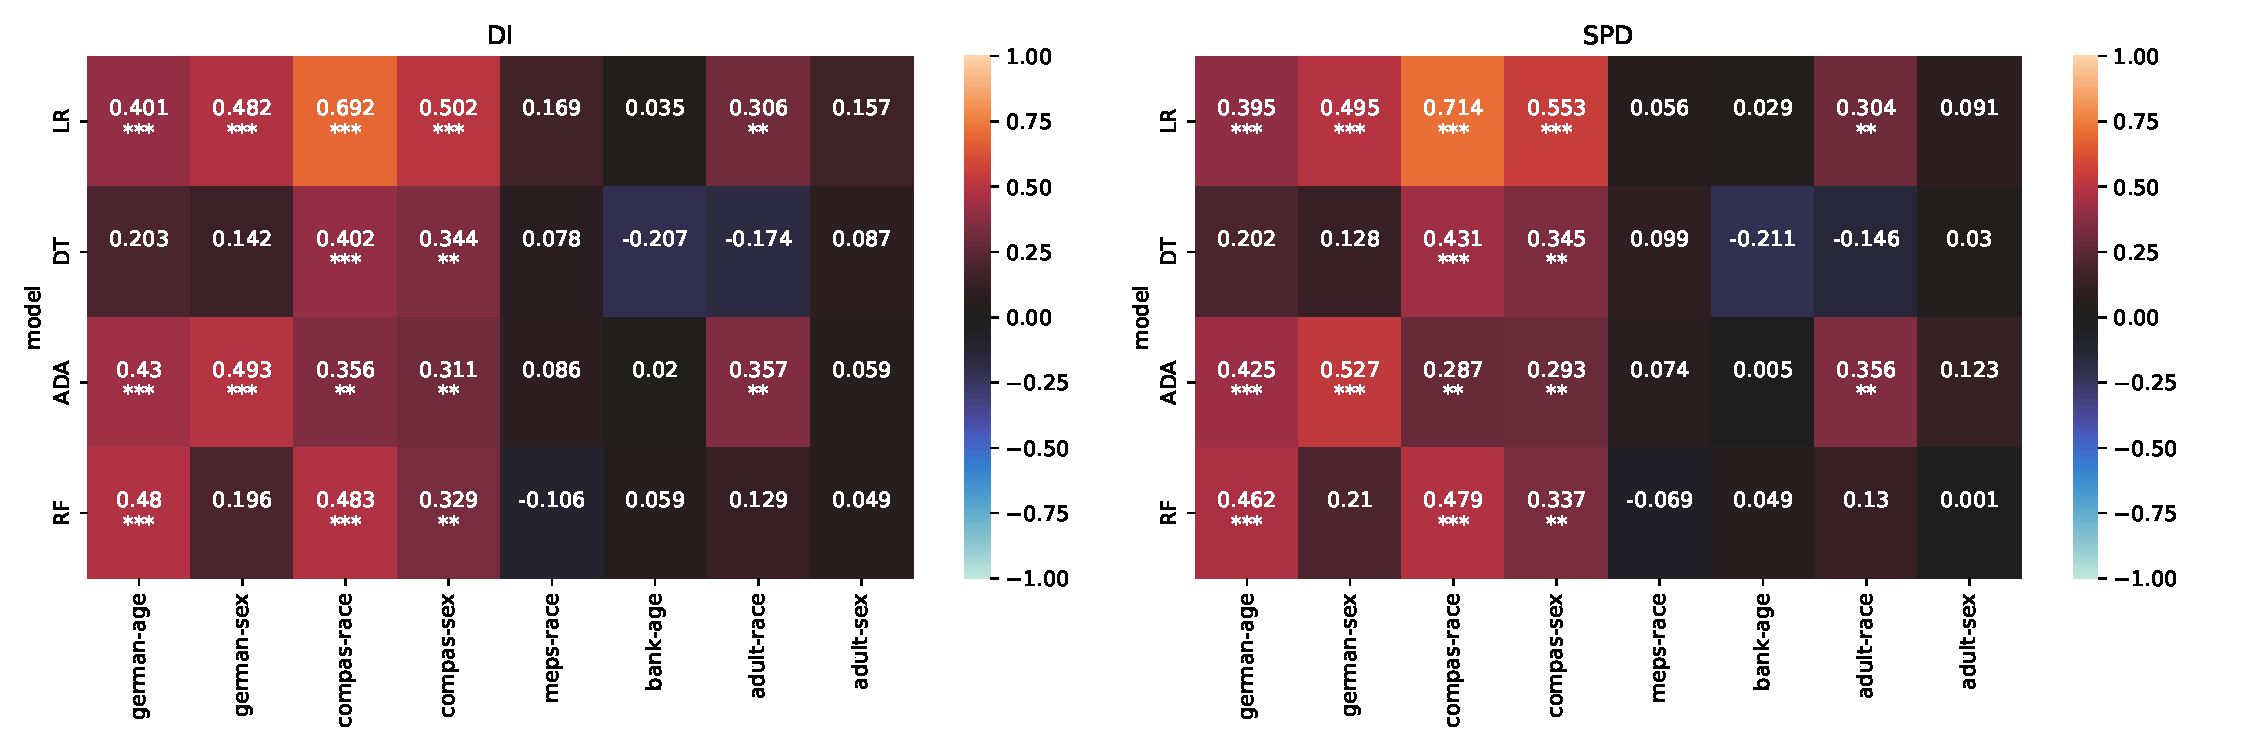
\includegraphics[width=\linewidth]{heatmap--corr--training-sets-frac.pdf}
  \caption{Correlation between DFM and MFM across all models and
  datasets using 60\% training data. The statistical significance is
  reported using asterisks at three $\alpha$ levels. ***: $p \le
  0.01$; **: $0.01 > p \le 0.05$; *: $0.05 > p \le 0.1$}
  \label{fig:heatmap--corr--training-sets-frac}
\end{figure}

Figure \ref{fig:heatmap--corr--training-sets-frac} shows the
correlation between the DFM and MFM across all models and datasets
when trained using 60\% of the original training set. The models used
in this study are represented along the y-axis and the datasets along
the x-axis. Darker colours indicate weaker correlation whereas
brighter colours indicate stronger correlation. Positive correlation
is indicated using hues of red while negative correlation is indicated
using hues of blue. The correlation between DFM and MFM for both
fairness metrics are shown separately. We primarily observe a positive
correlation between the DFM and MFM. This indicates that the DFM and
the MFM convey the same information as the distribution---and
consequently the fairness properties---of the underlying training
dataset changes.

\begin{figure}
  \centering
  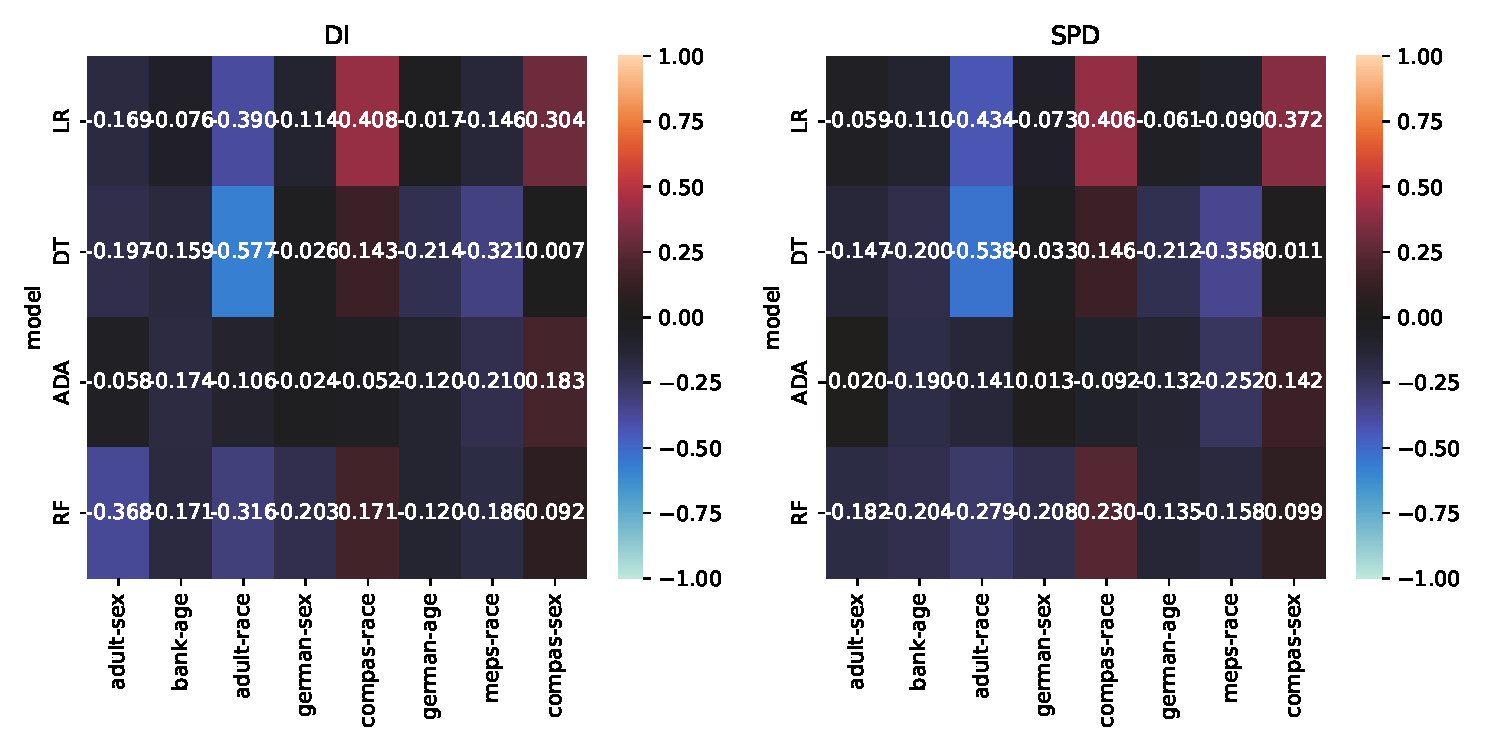
\includegraphics[width=\linewidth]{heatmap--corr--full-data.pdf}
  \caption{Correlation between DFM and MFM using the full training
  data. ***: $p \le 0.01$; **: $0.01 > p \le0.05$; *: $0.05 > p \le
  0.1$}
  \label{fig:heatmap--corr--full-data}
\end{figure}

In contrast to Figure \ref{fig:heatmap--corr--training-sets-frac},
Figure \ref{fig:heatmap--corr--full-data} shows the correlation
between DFM and MFM when the full training set is used. Due to lack of
significant change in the distribution of the training data, we
primarily observe darker colours indicating that the DFM and MFM are
not linearly related to one another anymore.

\highlight{\textbf{Answer to RQ1:} DFM and MFM are positively
correlated and thus convey the same information as the
distribution---and consequently the fairness properties---of the
underlying training dataset changes.}

\subsubsection{RQ2. How does the training sample size affect the
correlation between DFM and MFM?}\label{sec:results-corr-frac}

\begin{figure}
  \centering
  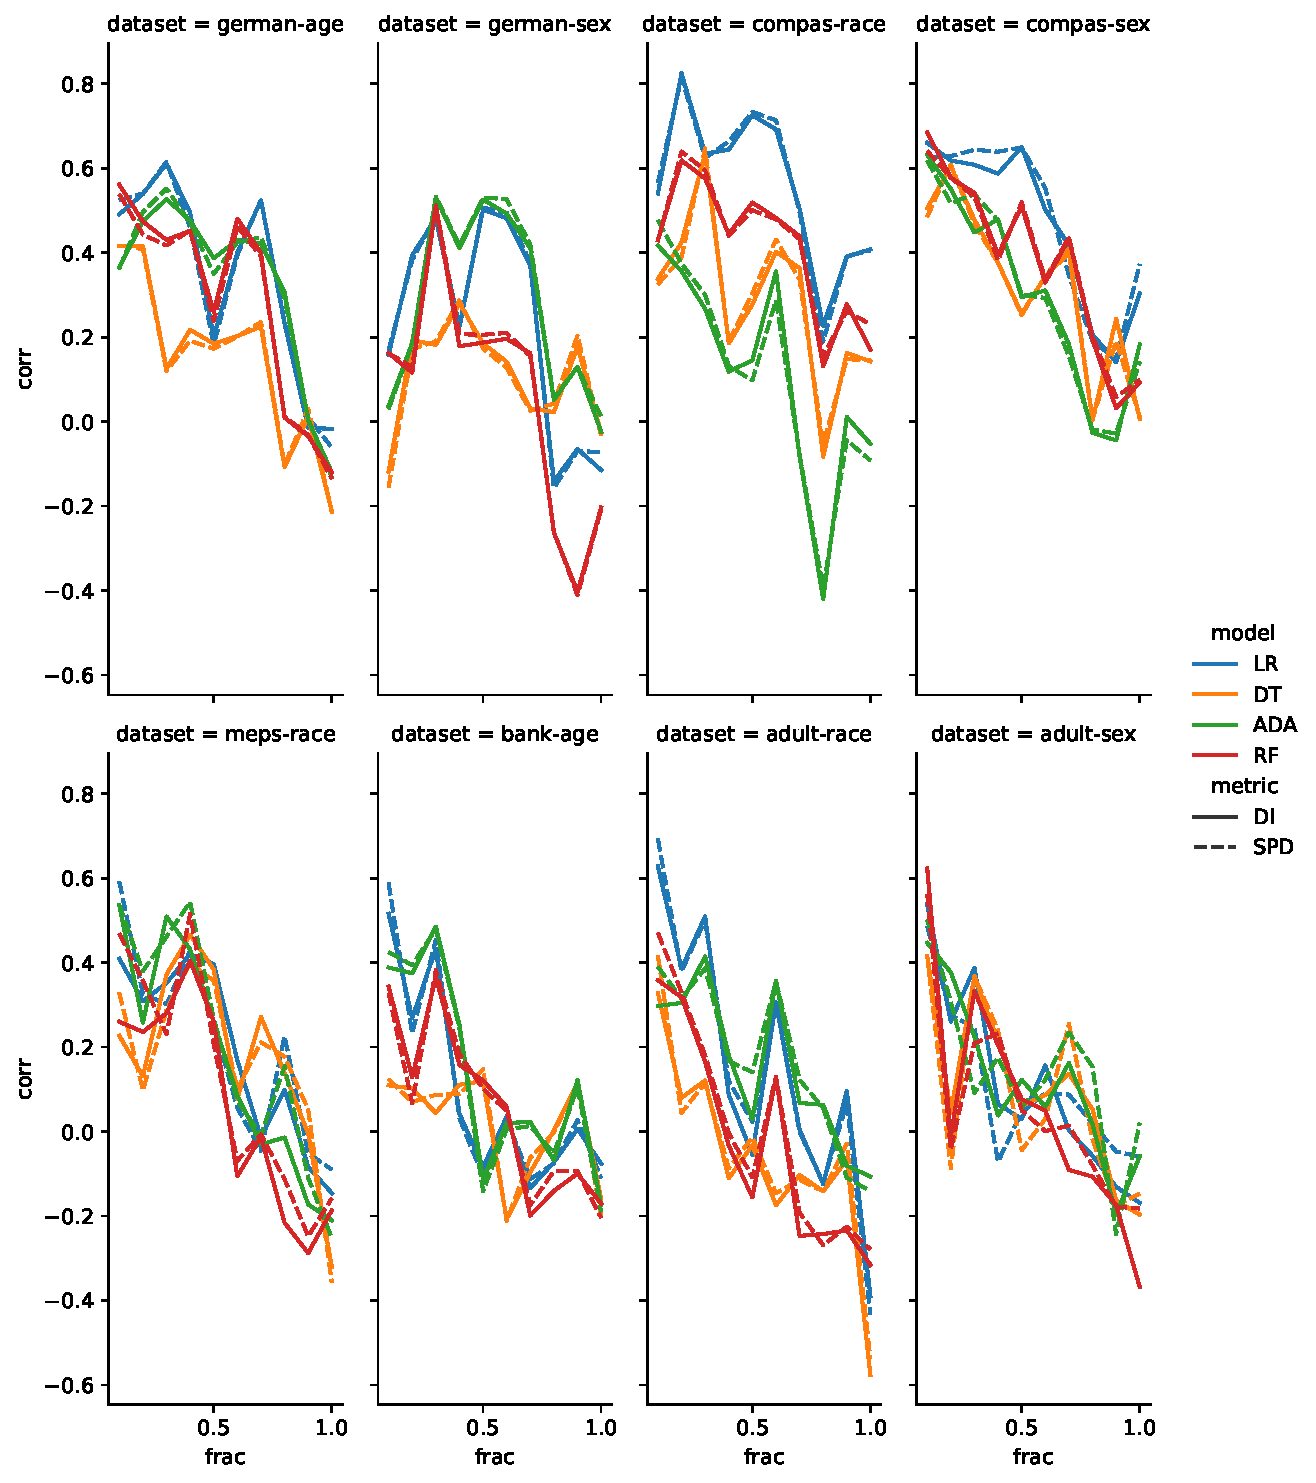
\includegraphics[width=0.95\linewidth]{lineplot--frac--corr.pdf}
  \caption{Distribution of correlation between DFM and MFM within
  various training sample sizes across all datasets and models.}
  \label{fig:lineplot--frac--corr}
\end{figure}

In Figure \ref{fig:heatmap--corr--training-sets-frac}, the correlation
in the smaller datasets are more positive compared to the larger
datasets when trained using 60\% of the original training data. When
the training data size is increased, the correlation in the datasets
decrease as observed in
Figure \ref{fig:heatmap--corr--full-data}. Based on these
observations, we hypothesise that the quantity of training data
influences the relationship between the DFM and MFM. Our hypothesis is
corroborated by Figure \ref{fig:lineplot--frac--corr} which shows the
distribution of the correlation between DFM and MFM within the various
training sample sizes, across all datasets and models. The x-axis
presents the training sample size and the y-axis presents the
correlation between the DFM and MFM. The colours represent the models
while the style of the line represents the two fairness metrics. Each
dataset is shown as a separate subplot. The overwhelming majority
shows that the correlation between the DFM and MFM decreases as we
increase the training sample size.

\highlight{\textbf{Answer to RQ2:} The training sample size has
a profound effect on the relationship between the DFM and MFM. The
correlation between the DFM and MFM decreases as we increase the
training sample size.}

\subsection{Training and Feature Sample Size
Experiments}\label{sec:results-training-feature-sets}
\subsubsection{RQ3. What is the relationship between DFM and MFM
across various training and feature sample sizes?}

\begin{figure}
  \centering
  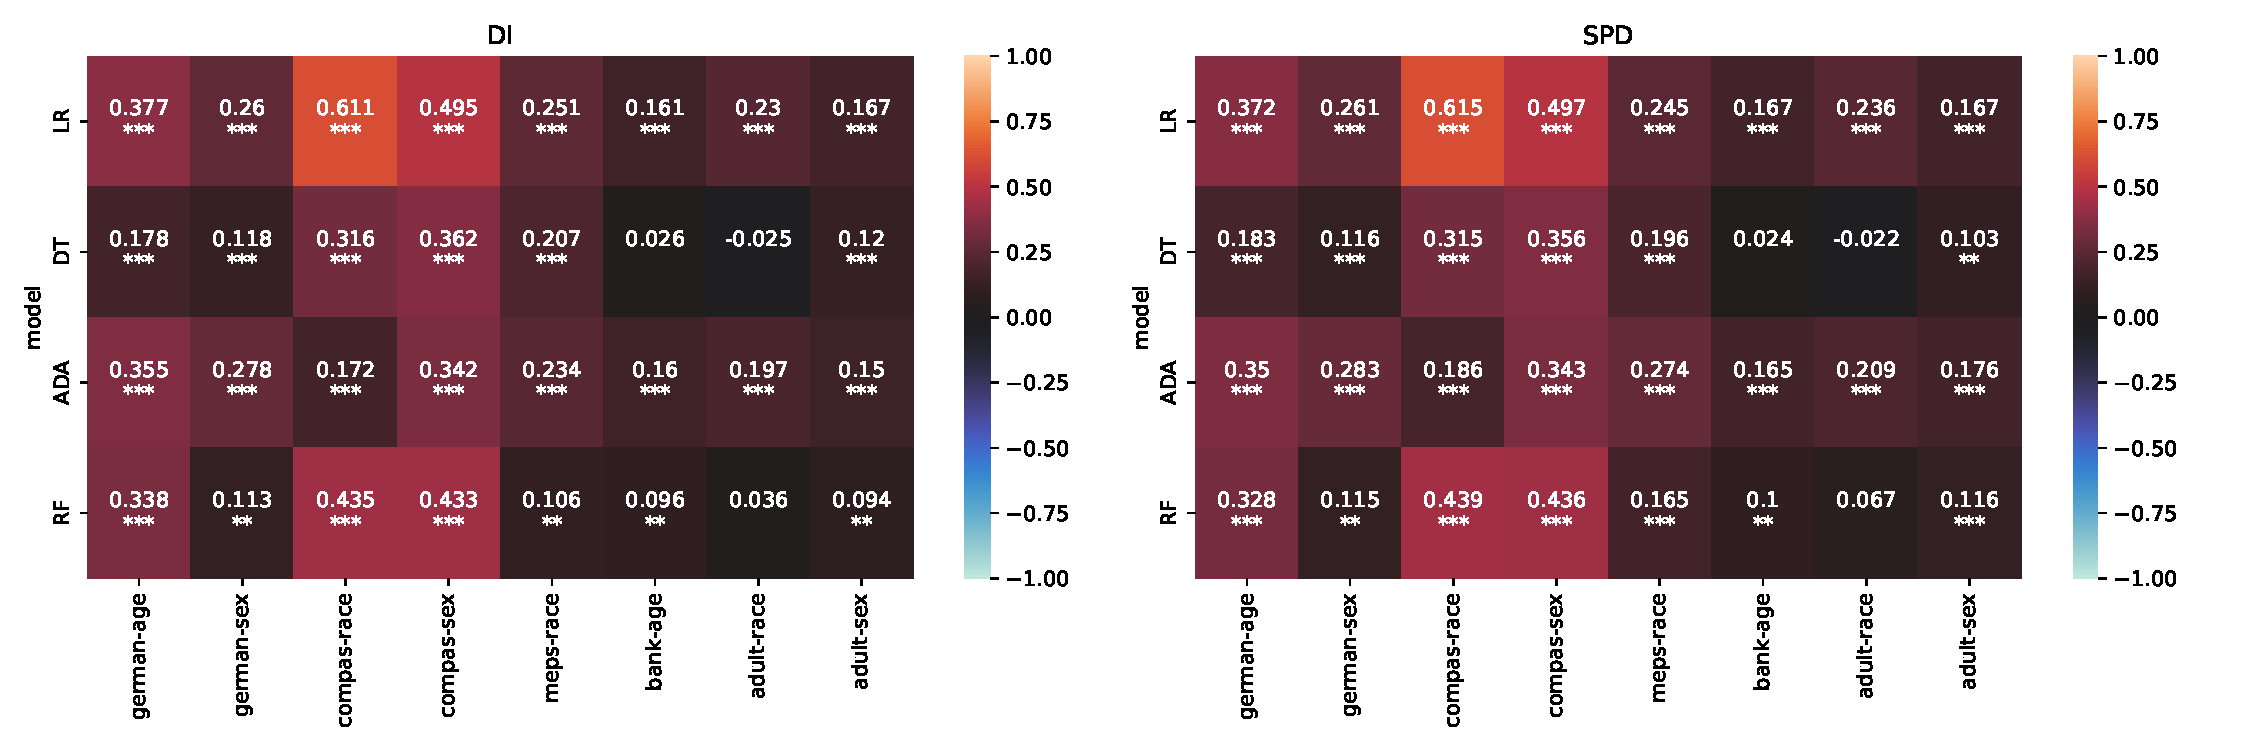
\includegraphics[width=\linewidth]{heatmap--corr--frac.pdf}
  \caption{Correlation between DFM and MFM acoss various training
  sample sizes. ***: $p \le 0.01$; **: $0.01 > p \le 0.05$; *: $0.05
  > p \le 0.1$}
  \label{fig:heatmap--corr--frac}
\end{figure}

\textbf{\emph{Training Sample Size.}} In this section we analyse the
relationship between DFM and MFM across varying training sample
sizes. In contrast to Section \ref{sec:results-corr-frac} where we
calculated the correlation between DFM and MFM within each training
sample size, here we calculate the correlation across all training
sample sizes. The correlation between the DFM and MFM is shown in
Figure \ref{fig:heatmap--corr--frac}. We primarily observe colours
indicating that the DFM and MFM convey similar information as the
training sample size changes.

\begin{figure}
  \centering
  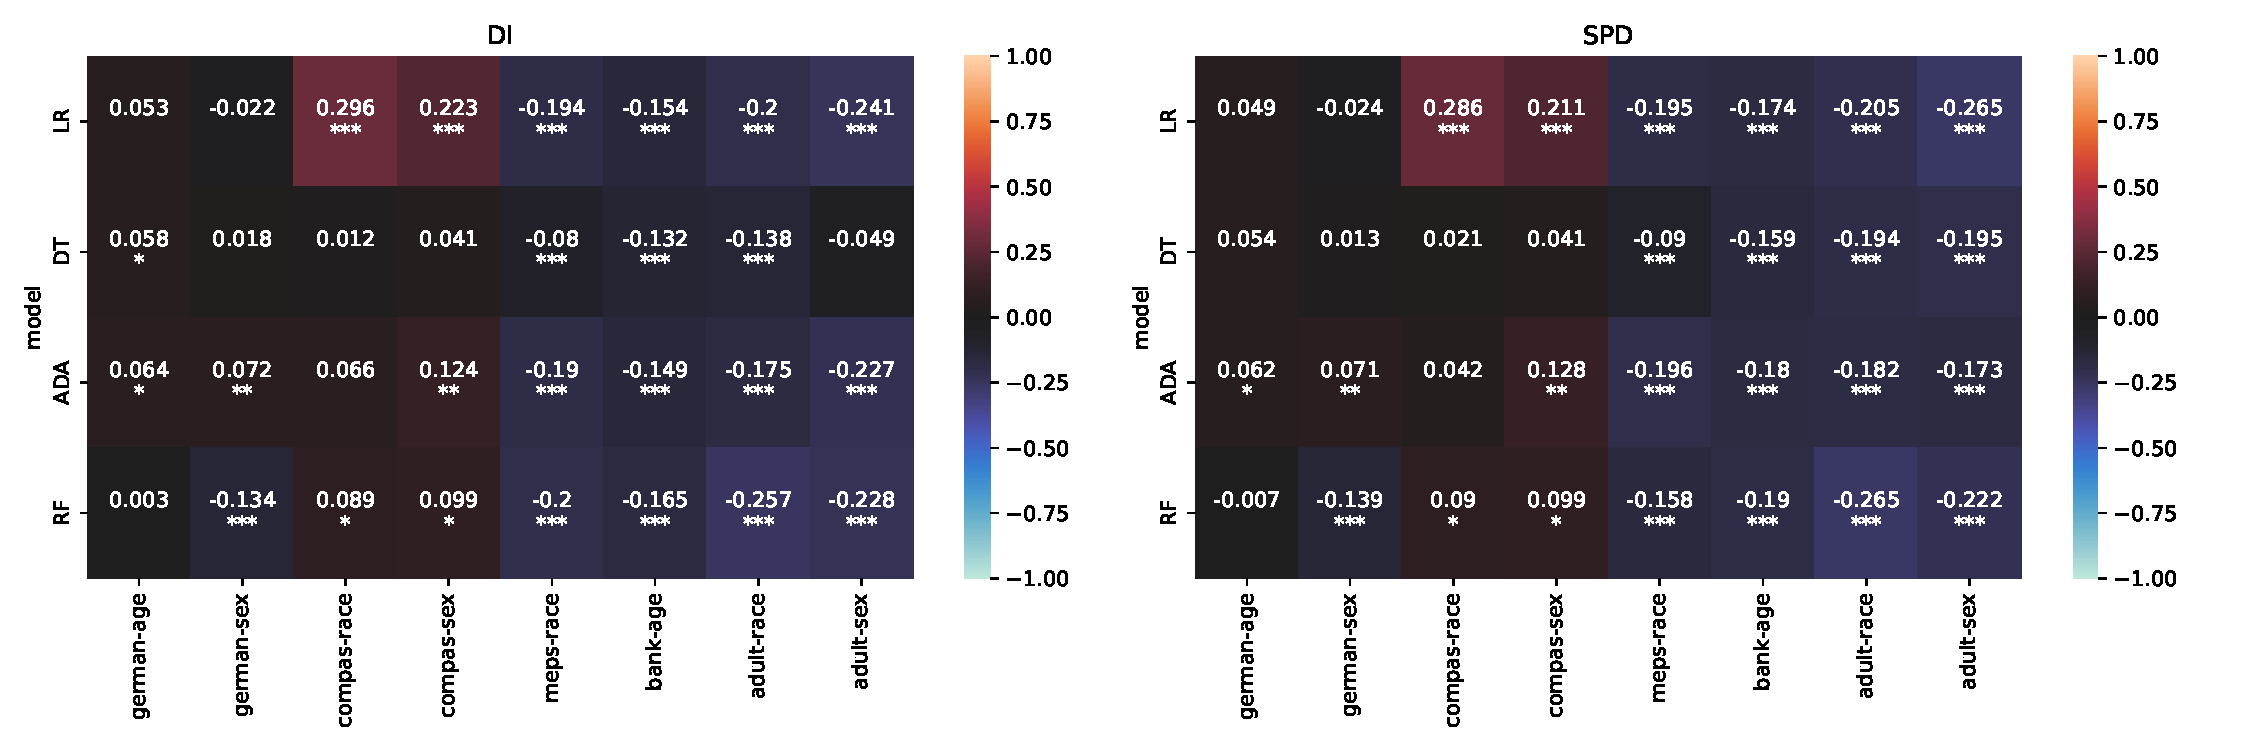
\includegraphics[width=\linewidth]{heatmap--corr--num-features.pdf}
  \caption{Correlation between DFM and MFM across various feature
  sample sizes. ***: $p \le 0.01$; **: $0.01 > p \le 0.05$; *: $0.05
  > p \le 0.1$}
  \label{fig:heatmap--corr--num-features}
\end{figure}

\textbf{\emph{Feature Sample Size.}} In this section we analyse the
relationship between the DFM and MFM across varying feature sample
sizes. In contrast to the training sample size experiment above, we
change the number of features in the training set and randomise the
feature order in each
iteration. Figure \ref{fig:heatmap--corr--num-features} presents the
correlation between the DFM and MFM across all feature sample
sizes. We primarily notice darker colours indicating that there is no
significant correlation between the DFM and MFM as the number of
features in the training dataset changes.

From Table \ref{tab:fairness-metrics}, we note that the feature sample
size does not affect the DFM thus explaining the lack of significant
correlation between the DFM and MFM. The larger datasets show a more
negative correlation. This however is due to the change in training
set distribution caused by the training-testing split within the 50
iterations as explained in Section \ref{sec:results-full}. This can
also be verified in Figure \ref{fig:lineplot--num-features--corr}
which shows the relationship between the correlation and the feature
sample sizes across all datasets and models. There is no discernible
relationship between the correlation and the feature sample size in
the top row containing datasets with a small training sample size and
varying feature sample size. A slight relationship can only be
observed in the bottom right subplots which contain datasets with
a large training sample size but small feature sample size.

\highlight{\textbf{Answer to RQ3:} DFM and MFM convey similar
information as the training sample size changes but not when the
feature sample size changes.}

\begin{figure}
  \centering
  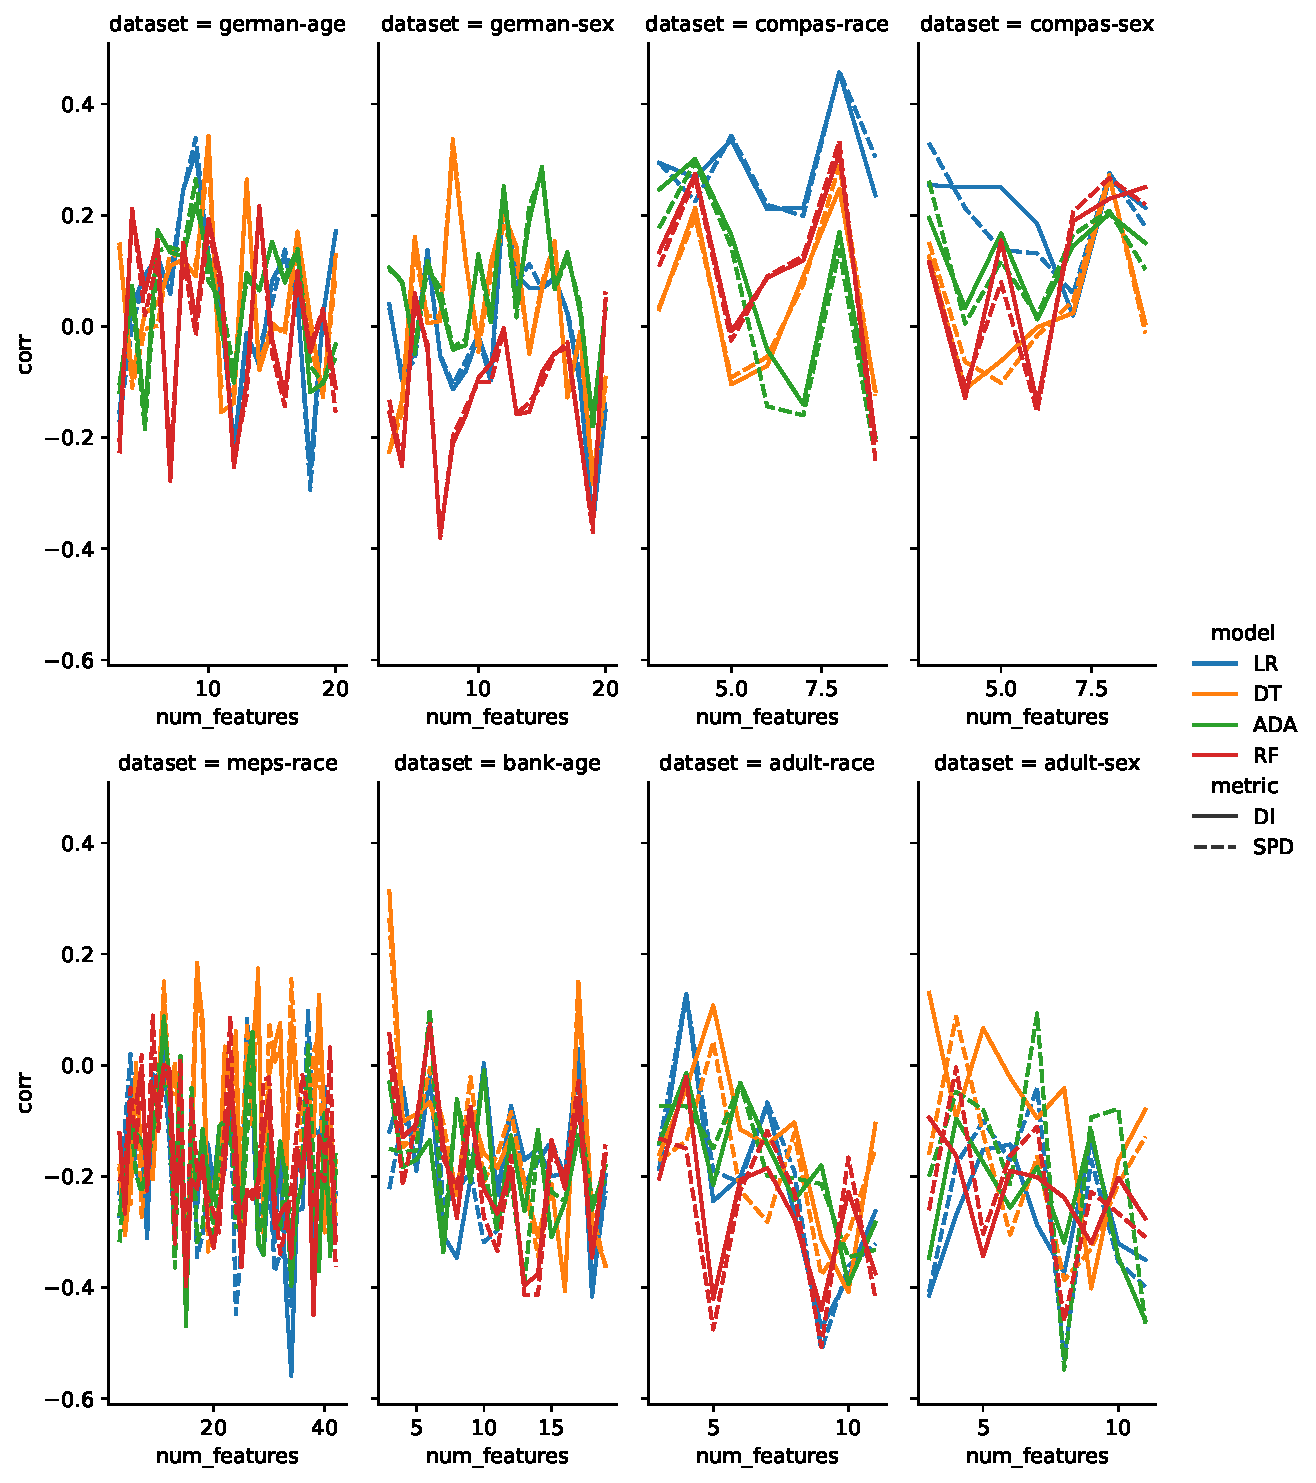
\includegraphics[width=0.95\linewidth]{lineplot--num-features--corr.pdf}
  \caption{Distribution of correlation between DFM and MFM across
  various features sample sizes.}
  \label{fig:lineplot--num-features--corr}
\end{figure}

\section{Implications}\label{sec:implications}
The implications of the results presented in Section \ref{sec:results}
along with their threats to validity are discussed in this section.

\subsection{Discussion}\label{sec:discuss}
\subsubsection{Data Drift}\label{sec:discuss-data-drift}

Results from RQ1 indicate that the DFM and MFM convey the same
information when the distribution and consequently the fairness
properties of the training data changes. ML systems running in
a production environment are often monitored to detect degradation in
model performance. A standard practise is to combine the data
encountered by the model in the production environment with its
predictions to create the training set for the next
iteration \cite{biessmann2021automated}. Since data reflects the real
world, change in its underlying distribution over time is eminent. Our
results indicate that DFM can be used as a early warning system to
identify fairness related data drifts in automated ML pipelines.

\subsubsection{Fairness, efficiency and performance trade-off}\label{sec:discuss-fair-eff-perf-trade}

Results from RQ2 indicate that the quantity of training data
profoundly influences the relationship between DFM and MFM. We
primarily see a positive correlation between the DFM and MFM in
smaller training sample sizes which indicates that the DFM and MFM
convey the same information. With sufficient training data, the
correlation starts to drop and eventually becomes negative. This
indicates that the models learn to make fairer predictions and are
able to circumvent the bias in the training data to a certain extent.

% TODO ellaborate what a positive correlation means; it means that
% when both DFM and MFM indicate presence of bias
Thus a positive correlation between the DFM and MFM may indicate lack
of sufficient training data. Under such circumstances, practitioners
can either choose to collect more data if possible or use bias
mitigation techniques to address the fairness issue.

A negative correlation between the DFM and MFM implies that the MFM
reported a lower value compared to the DFM. This does not however
guarantee the absence of bias in the
model. \citet{zhang2021ignorance} showed that in addition to the
quantity of training data, the quality itself affects the fairness of
ML systems. Introducing more data does not fix the bias in the model
if the final distribution remains biased.

Lower MFM compared to DFM also presents a trade-off between efficiency
and performance. A slight reduction in the training sample size, in
combination with appropriate bias mitigation techniques, can allow
practitioners to build fair ML systems with quicker training cycles at
the cost of negligible predictive
performance \cite{verdecchia2022data}. Engineering efficient, high
quality training data can reduce training cycles, development time and
ultimately project costs. Compounded over the entire duration that an
ML system stays in production along with the human effort required to
keep such a system operational, the benefits can be more than
substantial.

No correlation between DFM and MFM presents a trade-off between
fairness, efficiency and performance. Practitioners may opt for a more
efficient system by reducing the training sample size. However this
may reduce the predictive performance of the model and require more
engineering effort to mitigate the fairness issues in the system.
Alternatively, they may opt for more accurate predictions by using a
larger training sample size. A larger training size may mitigate some
of the bias in the training set at the cost of more compute.

\subsubsection{Test Reduction}\label{sec:discuss-test-red}

Results from RQ3 indicate that the DFM and MFM are positively
correlated and thus convey the same information when the training
sample size changes. DFM can therefore aid practitioners catch
fairness issues upstream and avoid execution costs of a full training
cycle. Considering the entire duration that an ML system is
operational, along with the multiple iterations it takes to test an ML
system, avoiding a full training cycle while evaluating its fairness
can be energy efficient and sustainable in the long run.

However the same test reduction cannot be made when experimenting with
the feature sample size of the training
set. \citet{zhang2021ignorance} showed that a larger feature sample
size typically improves the fairness of the model. To the best of our
knowledge, there are no fairness metrics that consider the influence
of other features on the fairness at the data level. Thus when
experimenting with the feature sample size, it is recommended that ML
practitioners evaluate the fairness both before and after training.

\subsubsection{Locating root cause of bias}\label{sec:discuss-root-cause-bias}

% TODO we have to mention chakraborty2021bias here; they do root cause
% of bias in ML!
Testing for fairness after training the model makes it very difficult
to identify where exactly the bias was introduced. Testing for
fairness both at the data (using DFM) and model (using MFM) level
provides a holistic view on the fairness of the entire system and can
aid practitioners identify the root cause of bias. If the DFM
indicates presence of bias, it can be an early indication of flaws in
the data collection process or flaws in the initial design of the
system itself. In the event that the DFM does not indicate bias but
the MFM does, practitioners can narrow down the cause of bias to the
learning algorithm itself and opt for in-processing or post-processing
bias mitigation techniques.

\subsubsection{Explaining fairness in decision trees}\label{sec:discuss-explain-fair-dt}

We consistently observe that Decision Trees (DTs) are able to make
fairer predictions with minimal effort. For instance, in
Figure \ref{fig:boxplot--dataset--di-spd--exp-full} we observe that
DTs report lower values for both fairness metrics across all
datasets. In Figure \ref{fig:lineplot--frac--corr} we observe that DTs
consistently report lower correlation between DFM and MFM compared to
other models. This indicates that DTs are able to mitigate the bias
present in the training data with a smaller training sample size and
continue to do so as the training same size changes. The above
observation pose an interesting line of query into examining why DTs
are able to produce fairer predictions using explainable AI
techniques.

\subsection{Threats to Validity}\label{sec:threats}

We do not apply the \emph{Bonferroni correction} to the correlation
analysis results. Although we report the $pvalue$ for completeness,
we do not base our implications only on the statistically significant
results. But rather on general trends observed in our analysis. For
all experiments, we additionally conduct linear regression analysis
using ordinary-least squares and check the coefficient of
determination ($R^2$) and the mean squared error (MSE) in the
residuals to evaluate the goodness of fit. 

% We set the MFM as the outcome (or dependent) variable $y$ and the
% DFM as the design (or independent) variable $x$. The linear
% regression results align with our findings from the correlation
% analysis. For the experiment in Section \ref{sec:results-full-rel},
% the $R^2$ in majority of the cases lie close to 0 indicating that
% the linear regression model is unable to explain the variability in
% the MFM using the DFM. For the experiment in
% Section \ref{sec:results-full-rel-dist}, the $R^2$ improves relative
% to the prior experiment thus reflecting the change we also observe
% in the correlation analysis.

% We use the spearman correlation implementation provided by
% scipy \ref{virtanen2020scipy} python library. The $pvalue$ provided
% by the current implementation however is not reliable for population
% size less than 500 experiments\footnote{See notes in the
% \href{https://docs.scipy.org/doc/scipy/reference/generated/scipy.stats.spearmanr.html}{library
% documentation}}. This is a threat to the experiments conducted in
% Section \ref{sec:results-full} since we only have 50 samples.

%% lack of correlation may arise from lack of significant bias in the
%% dataset; thus the DFM and MFM are just random and will never be
%% related; see german-sex for example

For the experiment conducted in Section \ref{sec:results-full-rel} the
selection of the training sample size of 60\% is a gross approximation
and may not be a good fit for all datasets used in this study. An
alternative albeit computationally more expensive solution would be to
identify this threshold individually for each dataset and update it
dynamically as its distribution changes.

\section{Conclusion}\label{sec:conclude}

Prior work in ML fairness testing evaluate fairness after the training
stage, using the predictions of the ML model. In contrast, this study
presents a more holistic approach by testing for fairness at two
distinct locations of the ML development lifecycle. We analyse the
relationship between model dependent and independent fairness metrics
empirically and find a linear relationship between data and model
fairness metrics when the distribution and the size of the training
data changes. Our results indicate that testing for fairness prior to
training can be a ``cheap'' and effective means of catching fairness
issues in the upstream stages of automated ML pipelines and aid
practitioners navigate the complex landscape of fairness testing. As
an extension of this study, we wish to evaluate the effectiveness of
DFM in real-world ML systems.

\bibliographystyle{named}
\bibliography{report}

\end{document}

